% ag2.rnw
% Time-stamp: c:/x/ag2.rnw

\documentclass[12pt]{article}\usepackage[]{graphicx}\usepackage[]{color}
%% maxwidth is the original width if it is less than linewidth
%% otherwise use linewidth (to make sure the graphics do not exceed the margin)
\makeatletter
\def\maxwidth{ %
  \ifdim\Gin@nat@width>\linewidth
    \linewidth
  \else
    \Gin@nat@width
  \fi
}
\makeatother

\definecolor{fgcolor}{rgb}{0.345, 0.345, 0.345}
\newcommand{\hlnum}[1]{\textcolor[rgb]{0.686,0.059,0.569}{#1}}%
\newcommand{\hlstr}[1]{\textcolor[rgb]{0.192,0.494,0.8}{#1}}%
\newcommand{\hlcom}[1]{\textcolor[rgb]{0.678,0.584,0.686}{\textit{#1}}}%
\newcommand{\hlopt}[1]{\textcolor[rgb]{0,0,0}{#1}}%
\newcommand{\hlstd}[1]{\textcolor[rgb]{0.345,0.345,0.345}{#1}}%
\newcommand{\hlkwa}[1]{\textcolor[rgb]{0.161,0.373,0.58}{\textbf{#1}}}%
\newcommand{\hlkwb}[1]{\textcolor[rgb]{0.69,0.353,0.396}{#1}}%
\newcommand{\hlkwc}[1]{\textcolor[rgb]{0.333,0.667,0.333}{#1}}%
\newcommand{\hlkwd}[1]{\textcolor[rgb]{0.737,0.353,0.396}{\textbf{#1}}}%

\usepackage{framed}
\makeatletter
\newenvironment{kframe}{%
 \def\at@end@of@kframe{}%
 \ifinner\ifhmode%
  \def\at@end@of@kframe{\end{minipage}}%
  \begin{minipage}{\columnwidth}%
 \fi\fi%
 \def\FrameCommand##1{\hskip\@totalleftmargin \hskip-\fboxsep
 \colorbox{shadecolor}{##1}\hskip-\fboxsep
     % There is no \\@totalrightmargin, so:
     \hskip-\linewidth \hskip-\@totalleftmargin \hskip\columnwidth}%
 \MakeFramed {\advance\hsize-\width
   \@totalleftmargin\z@ \linewidth\hsize
   \@setminipage}}%
 {\par\unskip\endMakeFramed%
 \at@end@of@kframe}
\makeatother

\definecolor{shadecolor}{rgb}{.97, .97, .97}
\definecolor{messagecolor}{rgb}{0, 0, 0}
\definecolor{warningcolor}{rgb}{1, 0, 1}
\definecolor{errorcolor}{rgb}{1, 0, 0}
\newenvironment{knitrout}{}{} % an empty environment to be redefined in TeX

\usepackage{alltt}

\usepackage{wright-knit}
\IfFileExists{upquote.sty}{\usepackage{upquote}}{}

\begin{document}

\title{Some title}
\author{Kevin Wright}
\maketitle
\thispagestyle{fancy}

% Setup stuff.


% ----------------------------------------------------------------------------
\section{Setup}
\begin{knitrout}
\definecolor{shadecolor}{rgb}{0.988, 0.988, 0.988}\color{fgcolor}\begin{kframe}
\begin{alltt}
\hlkwd{require}\hlstd{(}\hlstr{"agridat"}\hlstd{)}
\hlkwd{require}\hlstd{(}\hlstr{"asreml"}\hlstd{)}
\hlkwd{require}\hlstd{(}\hlstr{"lattice"}\hlstd{)}
\hlkwd{require}\hlstd{(}\hlstr{"latticeExtra"}\hlstd{)}
\hlnum{1}\hlopt{+}\hlnum{1}
\end{alltt}
\begin{Soutput}
[1] 2
\end{Soutput}
\end{kframe}
\end{knitrout}



Title: The agridat package is growing

Abstract

The agridat package is an extensive collection of
data sets that have been previously published in
books and journals, primarily from agricultural
experiments.  A sample of datasets in the package
are presented graphically with interpretive comments.

% ----------------------------------------------------------------------------
\section{}

\begin{knitrout}
\definecolor{shadecolor}{rgb}{0.988, 0.988, 0.988}\color{fgcolor}\begin{kframe}
\begin{alltt}
\hlstd{dat} \hlkwb{<-} \hlstd{lee.potatoblight}

\hlcom{# Note the progression to lower scores as time passes in each year}
\hlstd{skp} \hlkwb{<-} \hlkwd{c}\hlstd{(}\hlkwd{rep}\hlstd{(}\hlnum{0}\hlstd{,}\hlnum{10}\hlstd{),}
         \hlkwd{rep}\hlstd{(}\hlnum{0}\hlstd{,}\hlnum{7}\hlstd{),}\hlnum{1}\hlstd{,}\hlnum{1}\hlstd{,}\hlnum{1}\hlstd{,}
         \hlkwd{rep}\hlstd{(}\hlnum{0}\hlstd{,}\hlnum{8}\hlstd{),}\hlnum{1}\hlstd{,}\hlnum{1}\hlstd{,}
         \hlkwd{rep}\hlstd{(}\hlnum{0}\hlstd{,}\hlnum{6}\hlstd{),}\hlnum{1}\hlstd{,}\hlnum{1}\hlstd{,}\hlnum{1}\hlstd{,}\hlnum{1}\hlstd{,}
         \hlkwd{rep}\hlstd{(}\hlnum{0}\hlstd{,}\hlnum{5}\hlstd{),}\hlnum{1}\hlstd{,}\hlnum{1}\hlstd{,}\hlnum{1}\hlstd{,}\hlnum{1}\hlstd{,}\hlnum{1}\hlstd{,}
         \hlkwd{rep}\hlstd{(}\hlnum{0}\hlstd{,}\hlnum{5}\hlstd{),}\hlnum{1}\hlstd{,}\hlnum{1}\hlstd{,}\hlnum{1}\hlstd{,}\hlnum{1}\hlstd{,}\hlnum{1}\hlstd{,}
         \hlkwd{rep}\hlstd{(}\hlnum{0}\hlstd{,}\hlnum{6}\hlstd{),}\hlnum{1}\hlstd{,}\hlnum{1}\hlstd{,}\hlnum{1}\hlstd{,}\hlnum{1}\hlstd{,}
         \hlkwd{rep}\hlstd{(}\hlnum{0}\hlstd{,}\hlnum{5}\hlstd{),}\hlnum{1}\hlstd{,}\hlnum{1}\hlstd{,}\hlnum{1}\hlstd{,}\hlnum{1}\hlstd{,}\hlnum{1}\hlstd{,}
         \hlkwd{rep}\hlstd{(}\hlnum{0}\hlstd{,}\hlnum{5}\hlstd{),}\hlnum{1}\hlstd{,}\hlnum{1}\hlstd{,}\hlnum{1}\hlstd{,}\hlnum{1}\hlstd{,}\hlnum{1}\hlstd{,}
         \hlkwd{rep}\hlstd{(}\hlnum{0}\hlstd{,}\hlnum{5}\hlstd{),}\hlnum{1}\hlstd{,}\hlnum{1}\hlstd{,}\hlnum{1}\hlstd{,}\hlnum{1}\hlstd{,}\hlnum{1}\hlstd{)}
\hlkwd{desplot}\hlstd{(y} \hlopt{~} \hlstd{col}\hlopt{*}\hlstd{row}\hlopt{|}\hlstd{date, dat,} \hlkwc{main}\hlstd{=}\hlstr{"lee.potatoblight"}\hlstd{,}
        \hlkwc{layout}\hlstd{=}\hlkwd{c}\hlstd{(}\hlnum{10}\hlstd{,}\hlnum{11}\hlstd{),}\hlkwc{skip}\hlstd{=skp)}
\end{alltt}


{\ttfamily\noindent\color{warningcolor}{Warning: coercing argument of type 'double' to logical}}\end{kframe}

{\centering 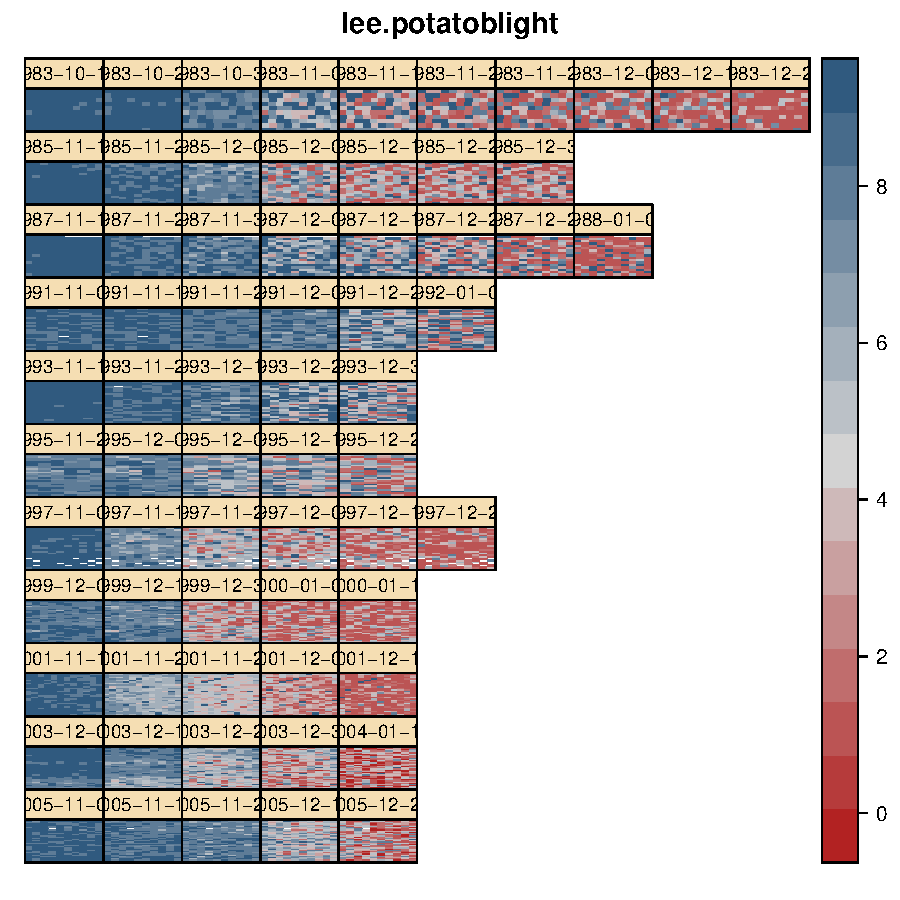
\includegraphics[width=\maxwidth]{figs/ag2-unnamed-chunk-21} 

}


\begin{kframe}\begin{alltt}
\hlcom{# 1983 only.  I.Hardy succumbs quickly}
\hlkwd{xyplot}\hlstd{(y} \hlopt{~} \hlstd{date}\hlopt{|}\hlstd{gen, dat,} \hlkwc{subset}\hlstd{=year}\hlopt{==}\hlnum{1983}\hlstd{,} \hlkwc{group}\hlstd{=rep,}
       \hlkwc{ylab}\hlstd{=}\hlstr{"Blight resistance score"}\hlstd{,} \hlkwc{main}\hlstd{=}\hlstr{"lee.potatoblight"}\hlstd{,} \hlkwc{as.table}\hlstd{=}\hlnum{TRUE}\hlstd{)}
\end{alltt}
\end{kframe}

{\centering 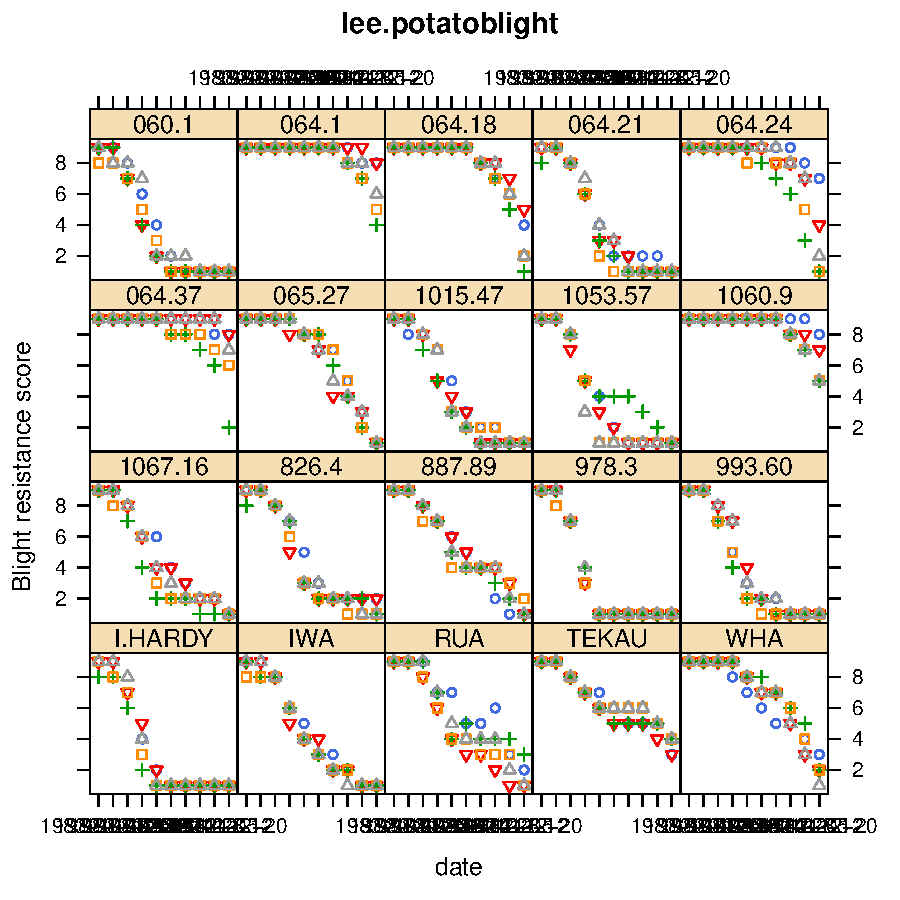
\includegraphics[width=\maxwidth]{figs/ag2-unnamed-chunk-22} 

}



\end{knitrout}

% ----------------------------------------------------------------------------

\pagebreak
\section{An informative prior}

\cite{harrison2012bayesian} used a Bayesian approach to model daidzein in soybean
samples.  In order to develop an informative prior for the distribution of
daidzen in soybean, 18 previous reports were compiled to a table listing the
source, number of samples tested, and the minimum and maximum observed
daidzein levels in the samples.  A lognormal distribution was fit for each
previous study, which was used to fill in the n-2 values between the minimum
and maximum.  The results are shown in the dotplot.  All observed/imputed data
were then used to fit a common lognormal distribution that can be used as an
informative prior.  This common prior is shown at the top of the dotplot.

\begin{knitrout}
\definecolor{shadecolor}{rgb}{0.988, 0.988, 0.988}\color{fgcolor}\begin{kframe}
\begin{Soutput}
     source number   min  max
1 Hutabarat      4 343.0 1400
2   Primomo      7 434.0  696
3  Morrison     14 696.0 1230
4  Berman-U     21 198.9 1274
5  Berman-A     21 361.5 1458
6  Lundry-U     13 274.9 1526
\end{Soutput}
\end{kframe}

{\centering 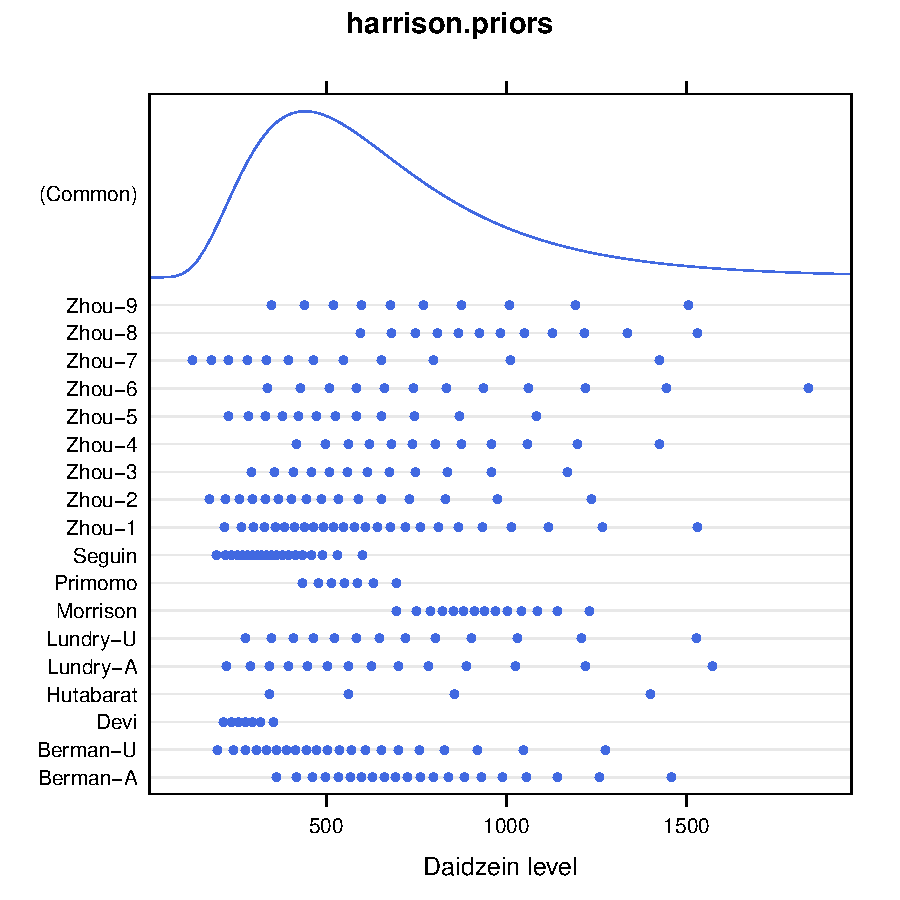
\includegraphics[width=\maxwidth]{figs/ag2-harrison} 

}



\end{knitrout}

% ----------------------------------------------------------------------------

\section*{Appendix}
This document was prepared \shorttoday\ with the following configuration:
\begin{kframe}
\begin{itemize}\raggedright
  \item R version 3.0.3 (2014-03-06), \verb|x86_64-w64-mingw32|
  \item Base packages: base, datasets, graphics, grDevices, grid, methods,
    stats, utils
  \item Other packages: agridat~1.9, asreml~3.0, knitr~1.5, lattice~0.20-29,
    latticeExtra~0.6-26, RColorBrewer~1.0-5, reshape2~1.4
  \item Loaded via a namespace (and not attached): compiler~3.0.3,
    evaluate~0.5.5, formatR~0.10, highr~0.3, plyr~1.8.1, Rcpp~0.11.1,
    stringr~0.6.2, tools~3.0.3
\end{itemize}
\end{kframe}

\bibliography{c:/x/notes/kw}
\end{document}
